\section{Algorithms}
Once we finished collecting and pre-processing the data, we thought about the different ways in which we can extract the required insights from it, thus we used to following NLP tools.


\subsection{Bag of Words - Term frequency}
We applied a Bag of Words model to determine the frequent appearance of terms in a "document" , in our case a document would be considered an entire game's data-set as we wish to compare the different games. We count the number of times every word appears in that game's entire data-set (both from twitter and Reddit combined). This has provided us with a simple metric to determine the use of certain words of interest in a community. These words of interest are divided into two groups of \emph{Neutral Sentiment Words} and \emph{Negative Sentiment Words} for each of the 3 terms we measure - \emph{Sexism}, \emph{Racism} and \emph{Trump-hate}.


\textcolor{red}{TODO - add lists of words here?!?!?}

\subsection{Word Embedding}


\subsection{Sentiment Analysis}
Sentiment Analysis \cite{liu2012sentiment} is a type of data mining, also known as opinion mining, that measures the inclination of people’s opinions through natural language processing (NLP), computational linguistics and text analysis. These methods used to extract and analyze subjective information from different sources like Twitter and Reddit in our case. 


We used in TextBlob library for sentiment analysis which return a tuple of form (polarity, subjectivity). The \emph{polarity} score is a float within the range [-1.0, 1.0] and it presents emotional state. Negative score represent negative emotional, 0 score represent neutral emotional and positive score represent positive emotional. The \emph{subjectivity} score is a float within the range [0.0, 1.0] and it describe if the post is subjective or objective,  where 0.0 is very objective and 1.0 is very subjective.
% Subjective sentence expresses some personal feelings, views, or beliefs. 

In our work we calculated polarity and subjectivity for every post in a specific community. We divided the results into three groups: Positive, Neutral and Negative polarity score. We calculate polarity average for each group, except for the neutral group whose average is known (0). Additionally, we calculate generally polarity average for all the posts in the community.


\subsection{Topic Modeling}
\textcolor{red}{TODO - review this}Topic-Modeling \cite{wallach2006topic} is the process of identifying topics in a set of documents. This can be useful for search engines, customer service automation, and any other instance where knowing the topics of documents is important. In our experiment we tried to get new information about the uniqe categories of each game and compare between the communities in each game hope to find difference, we ran topic model (unsupervised clustering) on every game and found categories with sexism and racism, .
% \begin{figure}[h]
% 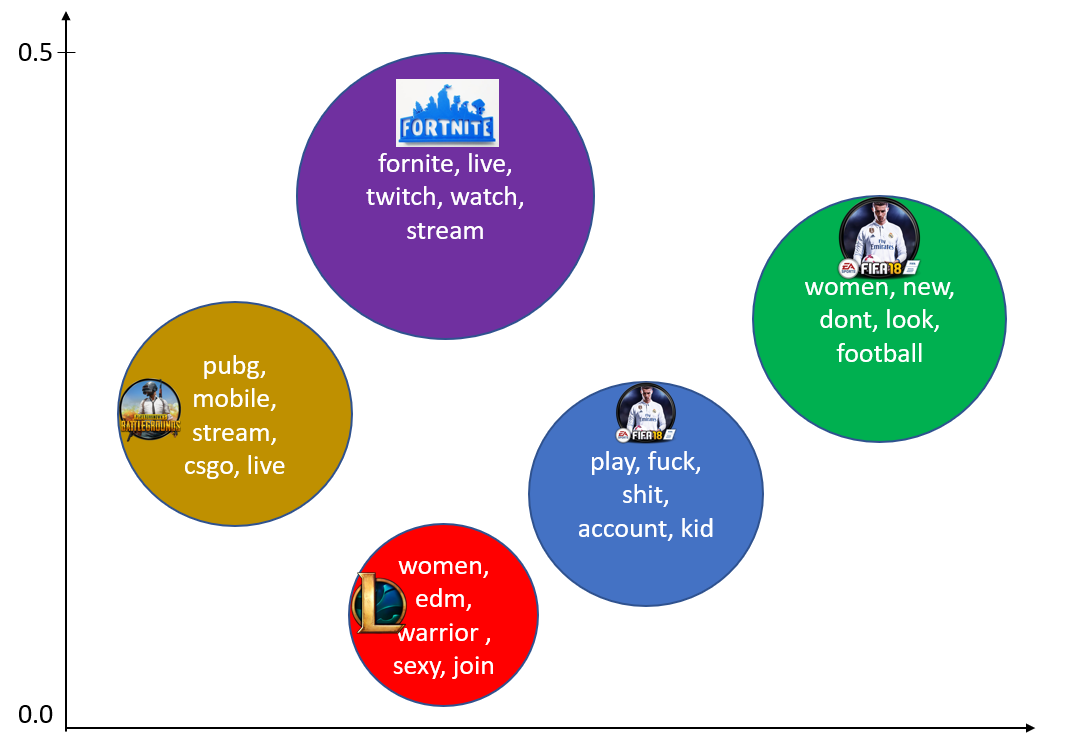
\includegraphics[width=0.5\textwidth]{Images/topicModel.PNG}
% \caption{\textcolor{red}{TODO - review this} The x-axis shows interesting categories that received high score (axis Y), for example we can see that fifa are sexist and cursing, on the other hand fortnite get the highest score on streaming category}
% \end{figure}

\subsection{Negativity Evaluation Metric}
 
